

\begin{figure}[!htbp]
    %\begin{wrapfigure}[32]{l}{0.5\columnwidth}
        %\resizebox{0.5\columnwidth}{!}{%
        \newcommand{\xdisposition}{0}
        \newcommand{\ydisposition}{0}
        \newcommand{\xtstep}{0.3}
        \newcommand{\ytstep}{0.7}
        \newcommand{\ybias}{-0.3 }
        \newcommand{\xstep}{2}
        \newcommand{\ystep}{-0.6}
        \newcommand{\xtscale}{0.8}
        \def\crossoutopacity{0.3}
        \def \numevents{29}
        \def\scale{0.8}
        \centering
    %    \resizebox{\columnwidth}{!}{%
        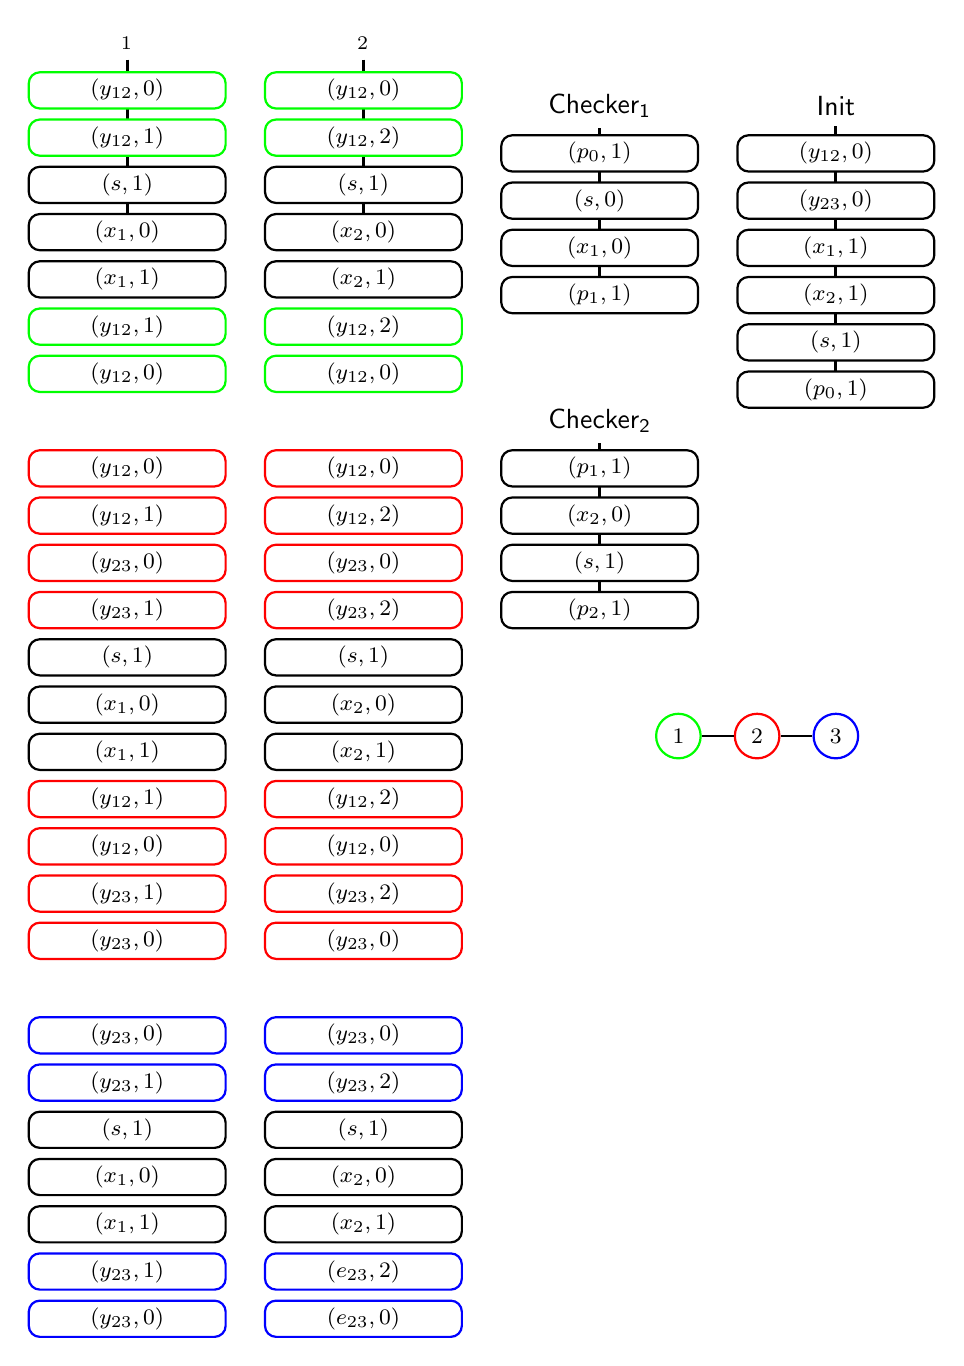
\begin{tikzpicture}[thick, font=\footnotesize,
        pre/.style={<-,shorten >= 2pt, shorten <=2pt, very thick},
        post/.style={->,shorten >= 3pt, shorten <=3pt,   thick},
        seqtrace/.style={line width=1},
        und/.style={very thick, draw=gray},
        virt/.style={circle,draw=black!50,fill=black!20, opacity=0}]
    
        \tikzstyle{event} = [rectangle, fill=white, inner sep=0, minimum height=4.6mm, minimum width=25mm, rounded corners]
    
    
        \node[] (S11) at (.5*\xstep,2*\ystep) {\normalsize $\Sel_{1}$};
        \node[] (S12) at (.5*\xstep,\numevents*\ystep) {};
        \draw[seqtrace] (S11) to (S12);
     
        \node[] (S21) at (2*\xstep,2*\ystep) {\normalsize $\Sel_{2}$};
        \node[] (S22) at (2*\xstep,\numevents*\ystep) {};
        
        
         \draw[seqtrace] (S21) to (S22);
         
    %%%%S1%%%%
       % \node[event, draw=black] (11) at (.5*\xstep, 1*\ystep + 0*\ybias) {$\rd(s, \top)$};
    
        \node[event, draw=green] (12) at (.5*\xstep, 3*\ystep + 0*\ybias) {$\rd(y_{12}, 0)$};
         \node[event, draw=green] (13) at (.5*\xstep, 4*\ystep + 0*\ybias) {$\wt(y_{12}, 1)$};
        
        \node[event, draw=black] (14) at (.5*\xstep, 5*\ystep + 0*\ybias) {$\rd(s, 1)$};
        \node[event, draw=black] (15) at (.5*\xstep, 6*\ystep + 0*\ybias) {$\wt(x_1, 0)$};
        \node[event, draw=black] (16) at (.5*\xstep, 7*\ystep + 0*\ybias) {$\wt(x_1, 1)$};
        
        \node[event, draw=green] (17) at (.5*\xstep, 8*\ystep + 0*\ybias) {$\rd(y_{12},1)$};
        \node[event, draw=green] (18) at (.5*\xstep, 9*\ystep + 0*\ybias) {$\wt(y_{12},0)$};
        
        
    
        \node[event, draw=red] (19) at (.5*\xstep, 11*\ystep + 0*\ybias) {$\rd(y_{12}, 0)$};
        \node[event, draw=red] (20) at (.5*\xstep, 12*\ystep + 0*\ybias) {$\wt(y_{12}, 1)$};
        \node[event, draw=red] (21) at (.5*\xstep, 13*\ystep + 0*\ybias) {$\rd(y_{23}, 0)$};
        \node[event, draw=red] (22) at (.5*\xstep, 14*\ystep + 0*\ybias) {$\wt(y_{23}, 1)$};
        
        
        
        
        
        \node[event, draw=black] (23) at (.5*\xstep, 15*\ystep + 0*\ybias) {$\rd(s, 1)$};
        \node[event, draw=black] (24) at (.5*\xstep, 16*\ystep + 0*\ybias) {$\wt(x_1, 0)$};
        \node[event, draw=black] (25) at (.5*\xstep, 17*\ystep + 0*\ybias) {$\wt(x_1, 1)$};
        
        
        \node[event, draw=red] (26) at (.5*\xstep, 18*\ystep + 0*\ybias) {$\rd(y_{12}, 1)$};
        \node[event, draw=red] (27) at (.5*\xstep, 19*\ystep + 0*\ybias) {$\wt(y_{12}, 0)$};
        \node[event, draw=red] (28) at (.5*\xstep, 20*\ystep + 0*\ybias) {$\rd(y_{23}, 1)$};
        \node[event, draw=red] (29) at (.5*\xstep, 21*\ystep + 0*\ybias) {$\wt(y_{23}, 0)$};
        
        
        
       \node[event, draw=blue] (31) at (.5*\xstep, 23*\ystep + 0*\ybias) {$\rd(y_{23}, 0)$};
        \node[event, draw=blue] (32) at (.5*\xstep, 24*\ystep + 0*\ybias) {$\wt(y_{23}, 1)$};
        \node[event, draw=black] (33) at (.5*\xstep, 25*\ystep + 0*\ybias) {$\rd(s, 1)$};
        \node[event, draw=black] (34) at (.5*\xstep, 26*\ystep + 0*\ybias) {$\wt(x_1, 0)$};
        \node[event, draw=black] (35) at (.5*\xstep, 27*\ystep + 0*\ybias) {$\wt(x_1, 1)$};\node[event, draw=blue] (36) at (.5*\xstep, 28*\ystep + 0*\ybias) {$\rd(y_{23}, 1)$};
        \node[event, draw=blue] (37) at (.5*\xstep, 29*\ystep + 0*\ybias) {$\wt(y_{23}, 0)$};
    
       
    %%%%S2%%%%%
    
    
    % \node[event, draw=black] (11) at (2*\xstep, 1*\ystep + 0*\ybias) {$\rd(s, \top)$};
    
        \node[event, draw=green] (12) at (2*\xstep, 3*\ystep + 0*\ybias) {$\rd(y_{12}, 0)$};
         \node[event, draw=green] (13) at (2*\xstep, 4*\ystep + 0*\ybias) {$\wt(y_{12}, 2)$};
        
        \node[event, draw=black] (14) at (2*\xstep, 5*\ystep + 0*\ybias) {$\rd(s, 1)$};
        \node[event, draw=black] (15) at (2*\xstep, 6*\ystep + 0*\ybias) {$\wt(x_2, 0)$};
        \node[event, draw=black] (16) at (2*\xstep, 7*\ystep + 0*\ybias) {$\wt(x_2, 1)$};
        
        \node[event, draw=green] (18) at (2*\xstep, 8*\ystep + 0*\ybias) {$\rd(y_{12},2)$};
        \node[event, draw=green] (19) at (2*\xstep, 9*\ystep + 0*\ybias) {$\wt(y_{12},0)$};
    
        \node[event, draw=red] (19) at (2*\xstep, 11*\ystep + 0*\ybias) {$\rd(y_{12}, 0)$};
        \node[event, draw=red] (20) at (2*\xstep, 12*\ystep + 0*\ybias) {$\wt(y_{12}, 2)$};
        
        \node[event, draw=red] (21) at (2*\xstep, 13*\ystep + 0*\ybias) {$\rd(y_{23}, 0)$};
       
        \node[event, draw=red] (22) at (2*\xstep, 14*\ystep + 0*\ybias) {$\wt(y_{23}, 2)$};
        
        \node[event, draw=black] (23) at (2*\xstep, 15*\ystep + 0*\ybias) {$\rd(s, 1)$};
        \node[event, draw=black] (24) at (2*\xstep, 16*\ystep + 0*\ybias) {$\wt(x_2, 0)$};
        \node[event, draw=black] (25) at (2*\xstep, 17*\ystep + 0*\ybias) {$\wt(x_2, 1)$};
        
        
        \node[event, draw=red] (26) at (2*\xstep, 18*\ystep + 0*\ybias) {$\rd(y_{12}, 2)$};
        \node[event, draw=red] (28) at (2*\xstep, 19*\ystep + 0*\ybias) {$\wt(y_{12}, 0)$};
        \node[event, draw=red] (29) at (2*\xstep, 20*\ystep + 0*\ybias) {$\rd(y_{23}, 2)$};
        \node[event, draw=red] (30) at (2*\xstep, 21*\ystep + 0*\ybias) {$\wt(y_{23}, 0)$};
        
        
       \node[event, draw=blue] (31) at (2*\xstep, 23*\ystep + 0*\ybias) {$\rd(y_{23}, 0)$};
        \node[event, draw=blue] (32) at (2*\xstep, 24*\ystep + 0*\ybias) {$\wt(y_{23}, 2)$};
        \node[event, draw=black] (33) at (2*\xstep, 25*\ystep + 0*\ybias) {$\rd(s, 1)$};
        \node[event, draw=black] (34) at (2*\xstep, 26*\ystep + 0*\ybias) {$\wt(x_2, 0)$};
        \node[event, draw=black] (35) at (2*\xstep, 27*\ystep + 0*\ybias) {$\wt(x_2, 1)$};
         \node[event, draw=blue] (36) at (2*\xstep, 28*\ystep + 0*\ybias) {$\rd(e_{23}, 2)$};
        \node[event, draw=blue] (37) at (2*\xstep, 29*\ystep + 0*\ybias) {$\wt(e_{23}, 0)$};
    
    %%%%%%%%%%%%%%%%%%%%%%%%%%%%%%%%%%%%%%%%%%%%%%%%%%%%%%
            
       
       \def \numevents{4}
      
       \begin{scope}[xshift=0cm,yshift=-2cm]
         
                \node[] (S11) at (3.5*\xstep,0) {\normalsize $\mathsf{Checker_1}$};
                \node[] (S12) at (3.5*\xstep, \numevents* \ystep) {};
            
                \draw[seqtrace] (S11) to (S12);
            
                
                \node[event, draw=black] (11) at (3.5*\xstep, 1*\ystep + 0*\ybias) {$\rd(p_{0}, 1)$};
                \node[event, draw=black] (12) at (3.5*\xstep, 2*\ystep + 0*\ybias) {$\wt(s, 0)$};
                
                \node[event, draw=black] (13) at (3.5*\xstep, 3*\ystep + 0*\ybias) {$\rd(x_1, 0)$};
                \node[event, draw=black] (13) at (3.5*\xstep, 4*\ystep + 0*\ybias) {$\wt(p_1, 1)$};
                
        
        \end{scope}
        
        \begin{scope}[xshift=0cm,yshift=-6cm]
         
                 \node[] (S11) at (3.5*\xstep,0) {\normalsize $\mathsf{Checker_2}$};
                \node[] (S12) at (3.5*\xstep, \numevents* \ystep) {};
            
                \draw[seqtrace] (S11) to (S12);
            
                
                \node[event, draw=black] (11) at (3.5*\xstep, 1*\ystep + 0*\ybias) {$\rd(p_{1}, 1)$};
              \node[event, draw=black] (12) at (3.5*\xstep, 2*\ystep + 0*\ybias) {$\rd(x_2, 0)$};                
                \node[event, draw=black] (13) at (3.5*\xstep, 3*\ystep + 0*\ybias) {$\wt(s, 1)$};                
                \node[event, draw=black] (13) at (3.5*\xstep, 4*\ystep + 0*\ybias) {$\wt(p_2, 1)$};
                
        
        \end{scope}
       
        
        \def \numevents{6}
          \begin{scope}[xshift=3cm,yshift=-2cm]
         
                \node[] (S11) at (3.5*\xstep,0) {\normalsize $\mathsf{Init}$};
                \node[] (S12) at (3.5*\xstep, \numevents* \ystep) {};
            
                \draw[seqtrace] (S11) to (S12);
            
                
                \node[event, draw=black] (11) at (3.5*\xstep, 1*\ystep + 0*\ybias) {$\wt(y_{12}, 0)$};
                \node[event, draw=black] (12) at (3.5*\xstep, 2*\ystep + 0*\ybias) {$\wt(y_{23}, 0)$};
                \node[event, draw=black] (13) at (3.5*\xstep, 3*\ystep + 0*\ybias) {$\wt(x_{1}, 1)$};
                \node[event, draw=black] (14) at (3.5*\xstep, 4*\ystep + 0*\ybias) {$\wt(x_2, 1)$};
                \node[event, draw=black] (15) at (3.5*\xstep, 5*\ystep + 0*\ybias) {$\wt(s, 1)$};
                \node[event, draw=black] (15) at (3.5*\xstep, 6*\ystep + 0*\ybias) {$\wt(p_0, 1)$};
        
        \end{scope}
        
    
                \begin{scope}[xshift=8cm,yshift=-10cm]
                \node[circle, draw=green, minimum size=.3cm] (1) {1};
                \node[circle, draw=red, minimum size=.3cm, right of=1] (2) {2};
                \node[circle, draw=blue, minimum size=.3cm, right of=2] (3) {3};
            
                % Edges
                \draw[-] (1) -- (2);
                \draw[-] (2) -- (3);
                \end{scope}
            
      
        \end{tikzpicture}   
        %}
        %}
        \caption{The $W[1]$-hardness reduction.}
        \label{fig:Example-w1}
    %\end{wrapfigure}
\end{figure}

